
\documentclass[a4paper,11pt]{article}  
\pagestyle{plain}
\usepackage{siunitx, dirtytalk, hyperref, nicefrac} 
\usepackage{graphicx,sectsty,longtable,tocloft,color,pdfpages,sidecap,subfig,array,eurosym}
 \captionsetup[figure]{labelfont={bf},name={Fig.},labelsep=period}

%\usepackage{refcheck} % places ??? for unused references in the PDF

\usepackage[english]{babel}
% smaller vertical spacing between references in bibliography
\let\OLDthebibliography\thebibliography
\renewcommand\thebibliography[1]{
  \OLDthebibliography{#1}
  \setlength{\parskip}{0pt}
  \setlength{\itemsep}{0pt plus 0.3ex}
}\usepackage{amsmath}
\usepackage{amsfonts}
\usepackage{amssymb}
%
% 2cm page margins (for A4)
%
\usepackage[left=2cm,right=2cm,top=2cm,bottom=2cm]{geometry}
\tolerance = 1000
\parindent 0cm
\parskip 2mm
%
% Section headings in Arial
%
\allsectionsfont{\sffamily}
%% Customise table of contents behaviour
\tocloftpagestyle{empty}
\renewcommand{\contentsname}{Table of Contents}
\renewcommand{\cfttoctitlefont}{\LARGE\bf\sffamily} 
% Add some width so section label A1.2.3.4 doesn't overlap with section title
\addtolength{\cftsecnumwidth}{3em}
\addtolength{\cftsubsecnumwidth}{3em}
\addtolength{\cftsubsubsecnumwidth}{3em}
%
% Some commonly used definitions
%
\def\urltilda{\kern -.15em\lower .7ex\hbox{\~{}}\kern .04em}
\def\urldot{\kern -.10em.\kern -.10em}
\def\urlhttp{http\kern -.10em\lower -.1ex\hbox{:}\kern -.12em\lower 0ex\hbox{/}\kern -.18em\lower 0ex\hbox{/}}
\def\xilinx{{\small\tt XILINX}}
\def\quarter{{$\frac{1}{4}$}}
\def\half{{$\frac{1}{2}$}}
\def\gm2{{\tt g-2}}
\def\geant{{\tt GEANT}}
\def\art{{\it art}}
\newcommand{\mue[1]}{{\tt Mu{#1}e}}
\newcommand{\gbp[1]}{\pounds\kern 0.08333em{#1}}
\newcommand{\eu[1]}{\euro\kern 0.08333em{#1}}
\newcommand{\usd[1]}{\$\kern 0.08333em{#1}}
%
\begin{document}
\pagenumbering{roman}
\thispagestyle{empty}
\begin{titlepage}
\begin{center}
	%\includegraphics[width=\textwidth]{fig/logo.png}
\end{center}
\begin{center}
	\vspace{1cm}
	{\huge Alignment:}\\
	\vspace{1.5cm}

	\vspace{6cm}
	{\LARGE\bf Gleb Lukicov}\\
	{\Large University College London}
	\vspace{4cm}
	\vfill
	\vspace{0.9cm}
	{\large October 31, 2017}
\end{center}
\end{titlepage}
\clearpage

\pagenumbering{arabic}
\thispagestyle{plain}
\section{Introduction} \label{sec:intro}

For parallel lines
\begin{equation}
R(x,M) = Track(x) - Hit(x,M) = \hat{m}z+\hat{c} - x(M)	
\end{equation}

\begin{equation}
\frac{ \partial R}{\partial m} = z	= DLC_2
\end{equation}

\begin{equation}
\frac{ \partial R}{\partial c} = 1	=DLC_1 = - DGL_1
\end{equation}

\clearpage

For general lines
\begin{equation}	
\mathrm{Residual}= R =\mathrm{Point \ To \ Line \ DCA} - \mathrm{Drift \ Circle \ Radius} = DCA(z,x,m,c) - r = \frac{ |c+mz-x| }  { \sqrt{m^2+1} } -r
\end{equation}


\begin{equation}
DLC_2 = \frac{ \partial R}{\partial m} = \frac{ (m^2+1)\cdot z\cdot(c+mz-x) - m\cdot |c+mz-x|^2 }{ (m^2+1)^{3/2} \cdot |c+mz-x|  } = \frac{\pm z}{\sqrt{m^2+1}} - \frac{m*|c+mz-x|}{(m^2+1)^{3/2}}
\end{equation}

\clearpage

PEDE Inputs (x mis.): 


\begin{equation}	
\mathrm{Residual}= R =\mathrm{Point \ To \ Line \ DCA} - \mathrm{Drift \ Circle \ Radius} = DCA(z,x,m,c) - r = \frac{ |c+mz-x| }  { \sqrt{m^2+1} } -r
\end{equation}


\begin{equation}	
\mathrm{Resolution} = \sigma = 150 \ \mu m = 0.015 \ \mathrm{cm}
\end{equation}

\begin{equation}	
\mathrm{Label}= \mathrm{Module \ Number}
\end{equation}

\begin{equation}
DLC_1 = \frac{\partial R}{\partial c} = \frac{ c+mz-x }  { \sqrt{m^2+1} \cdot |c+mz-x| }
\end{equation}

\begin{equation}
DLC_2 = \frac{ \partial R}{\partial m} = \frac{ (m^2+1)\cdot z\cdot(c+mz-x) - m\cdot |c+mz-x|^2 }{ (m^2+1)^{3/2} \cdot |c+mz-x|  }
\end{equation}

\begin{equation}	
DGL_1 = \frac{\partial R}{\partial x} = DLC_1 = - \frac{ c+mz-x }  { \sqrt{m^2+1} \cdot |c+mz-x| }
\end{equation}

\clearpage


PEDE Inputs for Circle Fit and Misalignment ($M$) along the beam direction ($z=z(M)=z+M$):


\begin{equation}	
\mathrm{Residual}= R =\mathrm{Point \ To \ Line \ DCA} - \mathrm{Drift \ Circle \ Radius} = DCA(z,x,m,c) - r = \frac{ |c+mz-x| }  { \sqrt{m^2+1} } -r
\end{equation}


\begin{equation}	
\mathrm{Resolution} = \sigma = 150 \ \mu m = 0.015 \ \mathrm{cm}
\end{equation}

\begin{equation}	
\mathrm{Label}= \mathrm{Module \ Number}
\end{equation}

\begin{equation}
DLC_1 = \frac{\partial R}{\partial c} = \frac{ c+mz-x }  { \sqrt{m^2+1} \cdot |c+mz-x| }
\end{equation}

\begin{equation}
DLC_2 = \frac{ \partial R}{\partial m} = \frac{ (m^2+1)\cdot z\cdot(c+mz-x) - m\cdot |c+mz-x|^2 }{ (m^2+1)^{3/2} \cdot |c+mz-x|  }
\end{equation}

\begin{equation}	
DGL_1 = \frac{\partial R}{\partial z} = \frac{ m(c+mz-x) }  { \sqrt{m^2+1} \cdot |c+mz-x| },
\end{equation}

 where $DGL_1 \rightarrow \pm \frac{m}{\sqrt{m^2+1}} \rightarrow \pm m$
(using TS expansion: $\pm \frac{m}{\sqrt{m^2+1}} \approx \pm m (1-\frac{1}{2}m^2) = \pm m - \frac{1}{2}m^3 \approx \pm m  $)

\clearpage

PEDE Inputs for Circle Fit and Misalignment ($M$) along the $x=x(M)=x+M$ and $z=z(M)=z+M$:
\begin{equation}	
\mathrm{Residual}= R =\mathrm{Point \ To \ Line \ DCA} - \mathrm{Drift \ Circle \ Radius} = DCA(z,x,m,c) - r = \frac{ |c+mz-x| }  { \sqrt{m^2+1} } -r
\end{equation}

\begin{equation}	
\mathrm{Resolution} = \sigma = 150 \ \mu m = 0.015 \ \mathrm{cm}
\end{equation}

\begin{equation}	
\mathrm{Label}= \mathrm{Module \ Number}
\end{equation}

\begin{equation}
DLC_1 = \frac{\partial R}{\partial c} = \frac{ c+mz-x }  { \sqrt{m^2+1} \cdot |c+mz-x| }
\end{equation}

\begin{equation}
DLC_2 = \frac{ \partial R}{\partial m} = \frac{ (m^2+1)\cdot z\cdot(c+mz-x) - m\cdot |c+mz-x|^2 }{ (m^2+1)^{3/2} \cdot |c+mz-x|  }
\end{equation}

\begin{equation}	
DGL_1 = \frac{\partial R}{\partial x} = DLC_1 = \frac{ c+mz-x }  { \sqrt{m^2+1} \cdot |c+mz-x| }
\end{equation}

\begin{equation}	
DGL_2 = \frac{\partial R}{\partial z} = \frac{ m(c+mz-x) }  { \sqrt{m^2+1} \cdot |c+mz-x| }
\end{equation}

 where $DGL_1 \rightarrow \pm \frac{1}{\sqrt{m^2+1}} \approx \pm 1 $ and $DGL_2 \rightarrow \pm \frac{m}{\sqrt{m^2+1}} \rightarrow \pm m$ \\
(using TS expansion: $\pm \frac{m}{\sqrt{m^2+1}} \approx \pm m (1-\frac{1}{2}m^2) = \pm m - \frac{1}{2}m^3 \approx \pm m  $)

\clearpage
\section{Generic Rotations:}

The aim of this section is to evaluate circle-fit residuals ($R$) with misalignment ($M$) as an anti-clockwise (AC) rotation ($\theta$) along the beam axis ($z=0$) through the detector centre. We now have 3 coordinate systems to refer to the straw positions (see Fig.~\ref{fig:theta}): \\
1) global coordinates ($z$, $x$) - relative to the \say{global} (0, 0). The derivatives of interest should be given w.r.t these coordinates. \\ 
2) local (\say{detector}) coordinates ($z_d$, $x_d$) in the \say{un-rotated} frame - relative to the centre of rotation of a detector, which is given by ($z^{centre}$, $x^{centre}$). These are orthogonal to the global coordinates. \\ 
3) local (\say{detector}) coordinates ($z'_{d}$, $x'_d$) in the rotated frame. Such that, for a centre of rotation ($z^{centre}_d$, $x^{centre}_d$) = ($z^{',centre}_{d}$, $x^{',centre}_d$) = (0,0), in the local coordinates.
\begin{figure}[!ht]
\centering
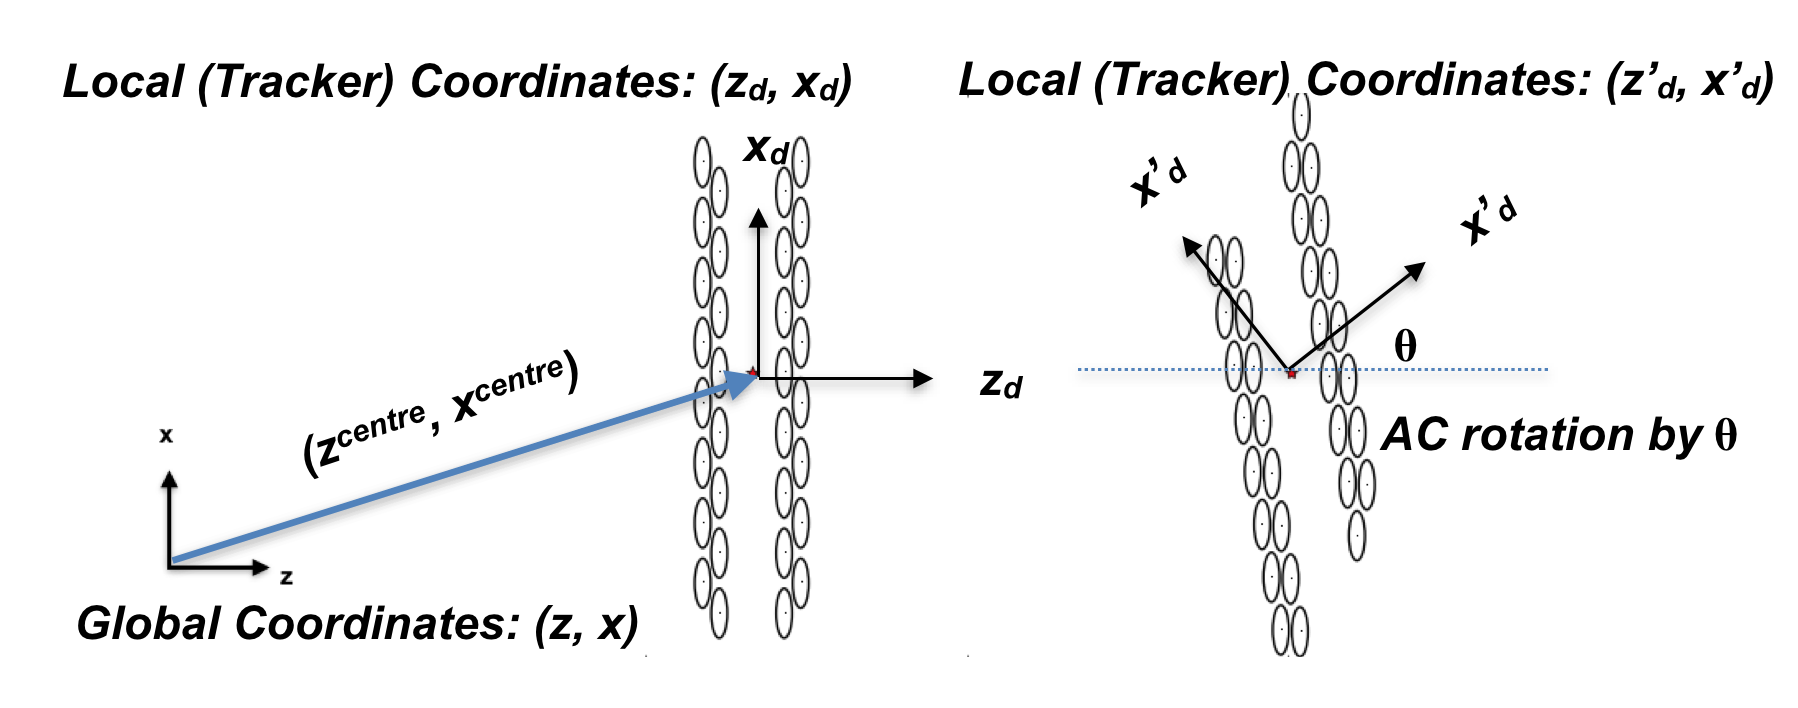
\includegraphics[width=0.9\linewidth]{imgLatex/theta.png}
\caption{The definition of the 3 coordinate systems.}
\label{fig:theta}
\end{figure}\\
With $z_d'=z_d(\theta)$ and $x'_d=x_d(\theta)$ transformations (the action of AC rotation) is given by
\begin{equation}
\begin{bmatrix}z_d'\\x_d'\\\end{bmatrix}=\begin{bmatrix}\cos \theta &-\sin \theta \\\sin \theta &\cos \theta \\\end{bmatrix} \begin{bmatrix}z_d\\x_d\\\end{bmatrix} = \begin{bmatrix}z_d\cos \theta -x_d\sin \theta \\z_d\sin \theta +x_d\cos \theta \\\end{bmatrix}.
\end{equation}
Then, we need to translate back to the global coordinates by
\begin{equation}
\begin{bmatrix}z\\x\\\end{bmatrix}=\begin{bmatrix}z_d'+z^{centre}\\x_d'+x^{centre}\\\end{bmatrix}=\begin{bmatrix}z_d\cos \theta -x_d\sin \theta + z^{centre} \\z_d\sin \theta +x_d\cos \theta + x^{centre} \\\end{bmatrix}. \label{eq:global}
\end{equation}
In the end, we need an expression for $\frac{\partial R}{\partial\theta}$ in terms of \textbf{reconstructed} (i.e. measured) parameters only. Essentially, 
\begin{equation}
\frac{\partial R}{\partial\theta} = \frac{\partial DCA(z,x,m,c)}{\partial\theta}= \frac{\partial DCA(z(\theta),x(\theta),m,c)}{\partial\theta},
\end{equation}
or, more generally, 
\begin{equation}
\frac{\partial R}{\partial\theta} = \frac{\partial R}{\partial m}\frac{\partial m}{\partial \theta} == \frac{\partial DCA(\theta)}{\partial\theta} = \frac{\partial DCA(m)}{\partial m}\frac{\partial m(\theta)}{\partial \theta},  \label{eq:partialRM}
\end{equation}
where $m$ represents a measurement (e.g. straw displacement in $z$ or $x$).
We can now write the equation for a residual (defined in Fig.~\ref{fig:res}) using Eq.~\ref{eq:global}
\begin{equation}
\begin{split}
\mathrm{Residual}= R =\mathrm{Point \ To \ Line \ DCA} - \mathrm{Drift \ Circle \ Radius} = DCA(z(\theta),x(\theta),m,c) - r = \\
= \frac{ |c+mz(\theta)-x(\theta)| }  { \sqrt{m^2+1} } -r = \frac{ |c+m(z_d\cos \theta -x_d\sin \theta + z^{centre})-(z_d\sin \theta +x_d\cos \theta + x^{centre})| }  { \sqrt{m^2+1} } -r=\\ = \frac{ |c+mz_d\cos \theta -mx_d\sin \theta + mz^{centre} -z_d\sin \theta - x_d\cos \theta - x^{centre}| }  { \sqrt{m^2+1} } -r.
\end{split}
\end{equation}
\clearpage
\begin{figure}[!ht]
\centering
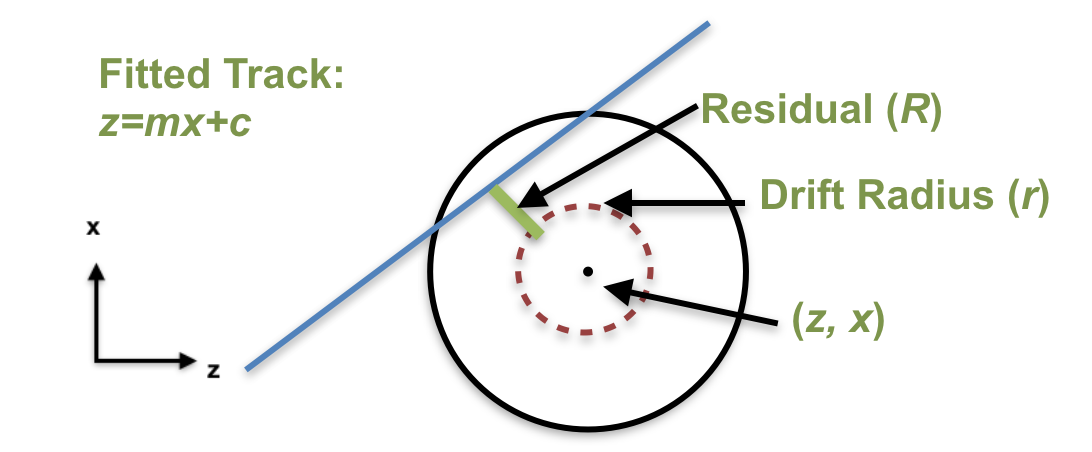
\includegraphics[width=0.6\linewidth]{imgLatex/res.png}
\caption{The pictorial representation of a residual.}
\label{fig:res}
\end{figure}
We can now use Eq.~\ref{eq:partialRM} to write the expression for the desired residual expressed without the use of truth parameters (i.e. $\theta$)
\begin{equation}
\begin{split}
\frac{\partial R}{\partial\theta} = \frac{\partial R}{\partial z}\frac{\partial z}{\partial \theta} + \frac{\partial R}{\partial x}\frac{\partial x}{\partial \theta} = \\ \frac{ m(c+mz-x) }  { \sqrt{m^2+1} \cdot |c+mz-x| } \times (-z_d\sin \theta - x_d\cos \theta) \ + \\ \frac{ c+mz-x }  { \sqrt{m^2+1} \cdot |c+mz-x| } \times (z_d\cos \theta - x_d\sin \theta) = \\
\frac{ m(c+mz-x) }  { \sqrt{m^2+1} \cdot |c+mz-x| } \times (-x'_d) + \\ \frac{ c+mz-x }  { \sqrt{m^2+1} \cdot |c+mz-x| } \times (z'_d) = \\
\frac{ m(c+mz-x) }  { \sqrt{m^2+1} \cdot |c+mz-x| } \times (-x + x^{centre}) + \\ \frac{ c+mz-x }  { \sqrt{m^2+1} \cdot |c+mz-x| } \times (z - z^{centre}).
\end{split}
\end{equation}
where all inputs come either from measurement or assumption of ideal geometry. This is form is familiar from previous studies of $M$ in $x$ and $z$, but with each respective $x$ or $z$ residual term multiplied by the difference between straw position and detector centre in $z$ or $x$, respectively. 

We are now ready to summarise the inputs to PEDE from a circle-fit with misalignment ($M$) as an anti-clockwise (AC) rotation ($\theta$) along the beam axis ($z=0$) through the detector centre.
\begin{equation}
\begin{split}
\mathrm{Residual} = R =\frac{ |c+mz-x| }  { \sqrt{m^2+1} } -r,
\end{split}
\end{equation}
where we have omitted the $\theta$ dependence of $x$ and $z$, as it is not a directly measured parameter.

\begin{equation}	
\mathrm{Resolution} = \sigma = 150 \ \mu m = 0.015 \ \mathrm{cm}.
\end{equation}

\begin{equation}	
\mathrm{Label}= \mathrm{Module \ Number} \times 10 + \mathrm{Global \ Parameter \ Number} = (e.g. \ 21, 31, \ etc.).
\end{equation}

\begin{equation}
DLC_1 = \frac{\partial R}{\partial c} = \frac{ c+mz-x }  { \sqrt{m^2+1} \cdot |c+mz-x| }.
\end{equation}

\begin{equation}
DLC_2 = \frac{ \partial R}{\partial m} = \frac{ (m^2+1)\cdot z\cdot(c+mz-x) - m\cdot |c+mz-x|^2 }{ (m^2+1)^{3/2} \cdot |c+mz-x|  }.
\end{equation}

\begin{equation}	
DGL_1 = \frac{\partial R}{\partial\theta} = 
\frac{ m(c+mz-x) }  { \sqrt{m^2+1} \cdot |c+mz-x| } \times (-x + x^{centre}) + \\ \frac{ c+mz-x }  { \sqrt{m^2+1} \cdot |c+mz-x| } \times (z - z^{centre}).
\end{equation}



\nocite{*}
\thispagestyle{plain}
%\begin{thebibliography}{100}

\bibitem{mp2} V. Blobel \textit{Software Alignment for Tracking Detectors}, Nucl. Instrum. Methods A, \textbf{556}, 5 (2006).

\bibitem{CMS} F.J.Rongaa et al., \textit{Tracking and Alignment in the CMS Detector}, Nucl. Phys. B, \textbf{172}, 202 (2007).

\bibitem{g-2_TDR} J. Grange et al., \textit{Muon (g-2) Technical Design Report}, arXiv:1501.06858 (2015).

\bibitem{art} A. Lyon et al., \textit{The art Event-Processing Framework}, \url{https://web.fnal.gov/project/ArtDoc/Pages/home.aspx} (2015).

\bibitem{Tom} T. Stuttard, \textit{The Development, Testing and Characterisation of a Straw Tracking Detector and Readout System for the Fermilab Muon g-2 Experiment}, PhD thesis, University College London (2017).

\bibitem{GBL} C. Kleinwort, \textit{General Broken Lines as Advanced Track Fitting Method}, Nucl. Instrum. Methods A \textbf{673}, 107 (2012).

\bibitem{GARFIELD} R. Veenhof, \textit{Garfield: Simulation of Gaseous Detectors}, \url{http://garfield.web. cern.ch/garfield} (2010).


\end{thebibliography}

%%%%% CLEAR DOUBLE PAGE!
\newpage{\pagestyle{empty}\cleardoublepage}
\addcontentsline{toc}{chapter}{\numberline{}\sf\bfseries{References}}
\end{document}